
%{{第四十二回}}{第四十二回}}

\chapter{蘅芜君兰言解疑癖\hspace{.5em}潇湘子雅谑补馀香}

{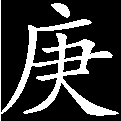
\includegraphics[width=3mm]{../Images/00004}  \kaishu 钗、玉名虽二个,人却一身,此幻笔也。今书至三十八回时,已过三分之一有馀,故写是回,使二人合而为一。请看黛玉逝后宝钗之文字,便知余言不谬矣。}

{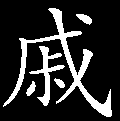
\includegraphics[width=3mm]{../Images/00005}  \kaishu 谁说诗书解误人,豪华相尚失天真。见得古人原立意,不正心身总莫论。}

话说他姊妹复进园来,吃过饭,大家散出,都无别话。

且说刘姥姥带着板儿,先来见凤姐儿,说:``明日一早定要家去了。虽住了两三天,日子却不多,把古往今来没见过的,没吃过的,没听见过的,都经验了。难得老太太和姑奶奶并那些小姐们,连各房里的姑娘们,都这样怜贫惜老照看我。我这一回去后没别的报答,惟有请些高香天天给你们念佛,保佑你们长命百岁的,就算我的心了。''凤姐儿笑道:``你别喜欢。都是为你,老太太也被风吹病了,睡着说不好过;我们大姐儿也着了凉,在那里发热呢。''刘姥姥听了,忙叹道:``老太太有年纪的人,不惯十分劳乏的。''凤姐儿道:``从来没像昨儿高兴。往常也进园子逛去,不过到一二处坐坐就回来了。昨儿因为你在这里,要叫你逛逛,一个园子倒走了多半个。大姐儿因为找我去,太太递了一块糕给他,谁知风地里吃了,就发起热来。''刘姥姥道:``小姐儿只怕不大进园子,生地方儿,小人儿家原不该去。比不得我们的孩子,会走了,那个坟圈子里不跑去。一则风扑了也是有的;二则只怕他身上干净,眼睛又净,或是遇见什么神了。依我说,给他瞧瞧祟书本子,仔细撞客着了。''一语提醒了凤姐儿,便叫平儿拿出《玉匣记》着彩明来念。彩明翻了一回念道:``八月二十五日,病者在东南方得遇花神。用五色纸钱四十张,向东南方四十步送之,大吉。''凤姐儿笑道:``果然不错,园子里头可不是花神!只怕老太太也是遇见了。''一面命人请两分纸钱来,着两个人来,一个与贾母送祟,一个与大姐儿送祟。果见大姐儿安稳睡了。{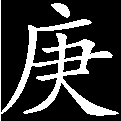
\includegraphics[width=3mm]{../Images/00004}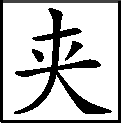
\includegraphics[width=3mm]{../Images/00012}\footnotesize \kaishu 岂真送了就安稳哉?盖妇人之心意皆如此,即不送,岂有一夜不睡之理?作者正描愚人之见耳。}

凤姐儿笑道:``到底是你们有年纪的人经历的多。我这大姐儿时常肯病,也不知是个什么原故。''刘姥姥道:``这也有的事。富贵人家养的孩子多太娇嫩,自然禁不得一些儿委曲;再他小人儿家,过于尊贵了,也禁不起。以后姑奶奶少疼他些就好了。''凤姐儿道:``这也有理。我想起来,他还没个名字,你就给他起个名字。一则借借你的寿;二则你们是庄家人,不怕你恼,到底贫苦些,你贫苦人起个名字,只怕压的住他。''{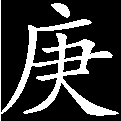
\includegraphics[width=3mm]{../Images/00004}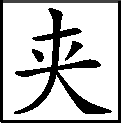
\includegraphics[width=3mm]{../Images/00012}\footnotesize \kaishu 一篇愚妇无理之谈,实是世间必有之事。}刘姥姥听说,便想了一想,笑道:``不知他几时生的?''凤姐儿道:``正是生日的日子不好呢,可巧是七月初七日。''刘姥姥忙笑道:``这个正好,就叫他是巧哥儿。这叫作`以毒攻毒,以火攻火'的法子。姑奶奶定要依我这名字,他必长命百岁。日后大了,各人成家立业,或一时有不遂心的事,必然是遇难成祥,逢凶化吉,却从这`巧'字上来。''{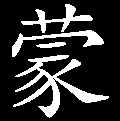
\includegraphics[width=3mm]{../Images/00006}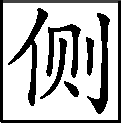
\includegraphics[width=3mm]{../Images/00011}\footnotesize \kaishu 作谶语以影射后文。}

凤姐儿听了,自是欢喜,忙道谢,又笑道:``只保佑他应了你的话就好了。''{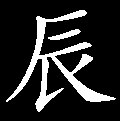
\includegraphics[width=3mm]{../Images/00009}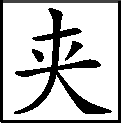
\includegraphics[width=3mm]{../Images/00012}\footnotesize \kaishu 伏后文。}说着叫平儿来吩咐道:``明儿咱们有事,恐怕不得闲儿。你这空儿把送姥姥的东西打点了,他明儿一早就好走的便宜了。''刘姥姥忙说:``不敢多破费了。已经遭扰了几日,又拿着走,越发心里不安起来。''{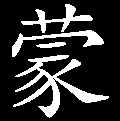
\includegraphics[width=3mm]{../Images/00006}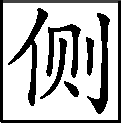
\includegraphics[width=3mm]{../Images/00011}\footnotesize \kaishu 世俗常态,逼真。}凤姐儿道:``也没有什么,不过随常的东西。好也罢,歹也罢,带了去,你们街坊邻舍看着也热闹些,也是上城一次。''只见平儿走来说:``姥姥过这边瞧瞧。''

刘姥姥忙赶了平儿到那边屋里,只见堆着半炕东西。平儿一一的拿与他瞧着,说道:``这是昨日你要的青纱一匹,奶奶另外送你一个实地子月白纱做里子。这是两个茧绸,作袄儿裙子都好。这包袱里是两匹绸子,年下做件衣裳穿。这是一盒子各样内造点心,也有你吃过的,也有你没吃过的,拿去摆碟子请客,比你们买的强些。这两条口袋是你昨日装瓜果子来的,如今这一个里头装了两斗御田粳米,熬粥是难得的;这一条里头是园子里果子和各样干果子。这一包是八两银子。这都是我们奶奶的。这两包每包里头五十两,共是一百两,是太太给的,叫你拿去或者作个小本买卖,或者置几亩地,以后再别求亲靠友的。''说着又悄悄笑道:``这两件袄儿和两条裙子,还有四块包头,一包绒线,可是我送姥姥的。衣裳虽是旧的,我也没大狠穿,你要弃嫌,我就不敢说了。''平儿说一样,刘姥姥就念一句佛,已经念了几千声佛了,又见平儿也送他这些东西,又如此谦逊,忙念佛道:``姑娘说那里话?这样好东西我还弃嫌!我便有银子也没处去买这样的呢。只是我怪臊的,收了又不好,不收又辜负了姑娘的心。''平儿笑道:``休说外话,咱们都是自己,我才这样。你放心收了罢,我还和你要东西呢。到年下,你只把你们晒的那个灰条菜干子和豇豆、扁豆、茄子、葫芦条儿各样干菜带些来,我们这里上上下下都爱吃。这个就算了,别的一概不要,别罔费了心。''刘姥姥千恩万谢答应了。平儿道:``你只管睡你的去。我替你收拾妥当了就放在这里,明儿一早打发小厮们雇辆车装上,不用你费一点心的。''

刘姥姥越发感激不尽,过来又千恩万谢的辞了凤姐儿,过贾母这一边睡了一夜,次早梳洗了就要告辞。因贾母欠安,众人都过来请安,出去传请大夫。一时婆子回大夫来了,老妈妈请贾母进幔子去坐。贾母道:``我也老了,那里养不出那阿物儿来,还怕他不成!不要放幔子,就这样瞧罢。''众婆子听了,便拿过一张小桌来,放下一个小枕头,便命人请。

一时只见贾珍、贾琏、贾蓉三个人将王太医领来。王太医不敢走甬路,只走旁阶,跟着贾珍到了阶矶上。早有两个婆子在两边打起帘子,两个婆子在前导引进去,又见宝玉迎了出来。只见贾母穿着青皱绸一斗珠的羊皮褂子,端坐在榻上,两边四个未留头的小丫鬟都拿着蝇帚漱盂等物;又有五六个老嬷嬷雁翅摆在两旁,碧纱厨后隐隐约约有许多穿红着绿戴宝簪珠的人。王太医便不敢抬头,忙上来请了安。贾母见他穿着六品服色,便知御医了,也便含笑问:``供奉好?''因问贾珍:``这位供奉贵姓?''贾珍等忙回:``姓王。''贾母道:``当日太医院正堂王君效,好脉息。''王太医忙躬身低头,含笑回说:``那是晚晚生家叔祖。''贾母听了,笑道:``原来这样,也是世交了。''一面说,一面慢慢的伸手放在小枕头上。老嬷嬷端着一张小杌,连忙放在小桌前,略偏些。王太医便屈一膝坐下,歪着头诊了半日,又诊了那只手,忙欠身低头退出。贾母笑说:``劳动了。珍儿让出去好生看茶。''

贾珍贾琏等忙答了几个``是'',复领王太医出到外书房中。王太医说:``太夫人并无别症,偶感一点风凉,究竟不用吃药,不过略清淡些,暖着一点儿,就好了。如今写个方子在这里,若老人家爱吃,便按方煎一剂吃,若懒待吃,也就罢了。''说着吃过茶写了方子。刚要告辞,只见奶子抱了大姐儿出来,笑说:``王老爷也瞧瞧我们。''王太医听说忙起身,就奶子怀中,左手托着大姐儿的手,右手诊了一诊,又摸了一摸头,又叫伸出舌头来瞧瞧,笑道:``我说姐儿又骂我了,只是要清清净净的饿两顿就好了,不必吃煎药,我送丸药来,临睡时用姜汤研开,吃下去就是了。''说毕作辞而去。

贾珍等拿了药方来,回明贾母原故,将药方放在桌上出去,不在话下。这里王夫人和李纨、凤姐儿、宝钗姊妹等见大夫出去,方从厨后出来。王夫人略坐一坐,也回房去了。

刘姥姥见无事,方上来和贾母告辞。贾母说:``闲了再来。''又命鸳鸯来,``好生打发刘姥姥出去。我身上不好,不能送你。''刘姥姥道了谢,又作辞,方同鸳鸯出来。

到了下房,鸳鸯指炕上一个包袱说道:``这是老太太的几件衣服,都是往年间生日节下众人孝敬的,老太太从不穿人家做的,收着也可惜,却是一次也没穿过的。{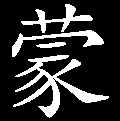
\includegraphics[width=3mm]{../Images/00006}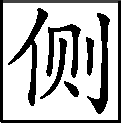
\includegraphics[width=3mm]{../Images/00011}\footnotesize \kaishu 写富贵常态,一笔作三五笔用,妙文。}昨日叫我拿出两套儿送你带去,或是送人,或是自己家里穿罢,别见笑。这盒子里是你要的面果子。这包子里是你前儿说的药:梅花点舌丹也有,紫金锭也有,活络丹也有,催生保命丹也有,每一样是一张方子包着,总包在里头了。这是两个荷包,带着顽罢。''说着便抽系子,掏出两个笔锭如意的锞子来给他瞧,又笑道:``荷包拿去,这个留下给我罢。''刘姥姥已喜出望外,早又念了几千声佛,听鸳鸯如此说,便说道:``姑娘只管留下罢。''鸳鸯见他信以为真,仍与他装上,笑道:``哄你顽呢,我有好些呢。留着年下给小孩子们罢。''{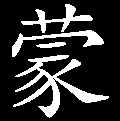
\includegraphics[width=3mm]{../Images/00006}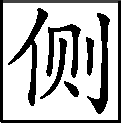
\includegraphics[width=3mm]{../Images/00011}\footnotesize \kaishu 逼真。}说着,只见一个小丫头拿了个成窑钟子来递与刘姥姥,``这是宝二爷给你的。''刘姥姥道:``这是那里说起。我那一世修了来的,今儿这样。''说着便接了过来。鸳鸯道:``前儿我叫你洗澡,换的衣裳是我的,你不弃嫌,我还有几件,也送你罢。''刘姥姥又忙道谢。鸳鸯果然又拿出两件来与他包好。刘姥姥又要到园中辞谢宝玉和众姊妹、王夫人等去。鸳鸯道:``不用去了。他们这会子也不见人,回来我替你说罢。闲了再来。''又命了一个老婆子,吩咐他:``二门上叫两个小厮来,帮着姥姥拿了东西送出去。''婆子答应了,又和刘姥姥到了凤姐儿那边一并拿了东西,在角门上命小厮们搬了出去,直送刘姥姥上车去了。不在话下。

且说宝钗等吃过早饭,又往贾母处问过安,回园至分路之处,宝钗便叫黛玉道:``颦儿跟我来,有一句话问你。''黛玉便同了宝钗,来至蘅芜苑中。进了房,宝钗便坐了笑道:``你跪下,我要审你。''{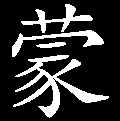
\includegraphics[width=3mm]{../Images/00006}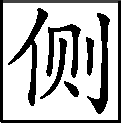
\includegraphics[width=3mm]{../Images/00011}\footnotesize \kaishu 严整。}黛玉不解何故,因笑道:``你瞧宝丫头疯了!审问我什么?''宝钗冷笑道:``好个千金小姐!好个不出闺门的女孩儿!满嘴说的是什么?你只实说便罢。''黛玉不解,只管发笑,心里也不免疑惑起来,口里只说:``我何曾说什么?你不过要捏我的错儿罢了。你倒说出来我听听。''宝钗笑道:``你还装憨儿。昨儿行酒令你说的是什么?我竟不知那里来的。''{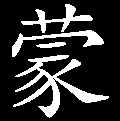
\includegraphics[width=3mm]{../Images/00006}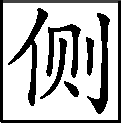
\includegraphics[width=3mm]{../Images/00011}\footnotesize \kaishu 何等爱惜。}

黛玉一想,方想起来昨儿失于检点,那《牡丹亭》、《西厢记》说了两句,不觉红了脸,便上来搂着宝钗,笑道:``好姐姐,原是我不知道随口说的。你教给我,再不说了。''{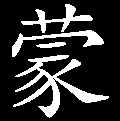
\includegraphics[width=3mm]{../Images/00006}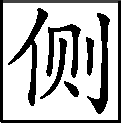
\includegraphics[width=3mm]{../Images/00011}\footnotesize \kaishu 真能受教。尊重之态,姣痴之情,令人爱煞!}宝钗笑道:``我也不知道,听你说的怪生的,所以请教你。''黛玉道:``好姐姐,你别说与别人,我以后再不说了。''宝钗见他羞得满脸飞红,满口央告,便不肯再往下追问,因拉他坐下吃茶,{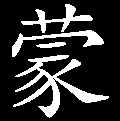
\includegraphics[width=3mm]{../Images/00006}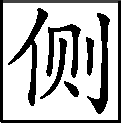
\includegraphics[width=3mm]{../Images/00011}\footnotesize \kaishu 若无下文,自己何由而知?笔下一丝不露痕迹中补足,存小姐身分,颦儿不得反问。}款款的告诉他道:``你当我是谁,我也是个淘气的。从小七八岁上也够个人缠的。我们家也算是个读书人家,祖父手里也爱藏书。先时人口多,姊妹弟兄都在一处,都怕看正经书。弟兄们也有爱诗的,也有爱词的,诸如这些《西厢》《琵琶》以及`元人百种',无所不有。{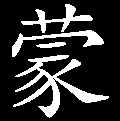
\includegraphics[width=3mm]{../Images/00006}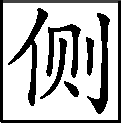
\includegraphics[width=3mm]{../Images/00011}\footnotesize \kaishu 藏书家当留意。}他们是偷背着我们看,我们却也偷背着他们看。后来大人知道了,打的打,骂的骂,烧的烧,才丢开了。所以咱们女孩儿家不认得字的倒好。男人们读书不明理,尚且不如不读书的好,何况你我。就连作诗写字等事,原不是你我分内之事,究竟也不是男人分内之事。男人们读书明理,辅国治民,这便好了。{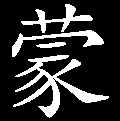
\includegraphics[width=3mm]{../Images/00006}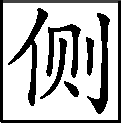
\includegraphics[width=3mm]{../Images/00011}\footnotesize \kaishu 作者一片苦心,代佛说法,代圣讲道,看书者不可轻忽。}只是如今并不听见有这样的人,读了书倒更坏了。这是书误了他,可惜他也把书遭塌了,所以竟不如耕种买卖,倒没有什么大害处。你我只该做些针黹纺织的事才是,偏又认得了字,既认得了字,不过拣那正经的看也罢了,最怕见了些杂书,移了性情,就不可救了。''一席话,说的黛玉垂头吃茶,心下暗伏,只有答应``是''的一字。{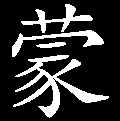
\includegraphics[width=3mm]{../Images/00006}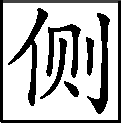
\includegraphics[width=3mm]{../Images/00011}\footnotesize \kaishu 结得妙。}

忽见素云进来说:``我们奶奶请二位姑娘商议要紧的事呢。二姑娘、三姑娘、四姑娘、史姑娘、宝二爷都在那里等着呢。''宝钗道:``又是什么事?''黛玉道:``咱们到了那里就知道了。''说着便和宝钗往稻香村来,果见众人都在那里。

李纨见了他两个,笑道:``社还没起,就有脱滑的了,四丫头要告一年的假呢。''黛玉笑道:``都是老太太昨儿一句话,又叫他画什么园子图儿,惹得他乐得告假了。''探春笑道:``也别要怪老太太,都是刘姥姥一句话。''林黛玉忙笑道:``可是呢,都是他一句话。他是那一门子的姥姥,直叫他是个`母蝗虫'就是了。''说着大家都笑起来。宝钗笑道:``世上的话,到了凤丫头嘴里也就尽了。幸而凤丫头不认得字,不大通,不过一概是市俗取笑。更有颦儿这促狭嘴,他用`春秋'的法子,将市俗的粗话,撮其要,删其繁,再加润色比方出来,一句是一句。{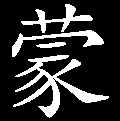
\includegraphics[width=3mm]{../Images/00006}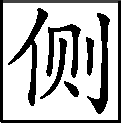
\includegraphics[width=3mm]{../Images/00011}\footnotesize \kaishu 触目惊心,请自回思。}这`母蝗虫'三字,把昨儿那些形景都现出来了。亏他想的倒也快。''众人听了,都笑道:``你这一注解,也就不在他两个以下。''

李纨道:``我请你们大家商议,给他多少日子的假。我给了他一个月他嫌少,你们怎么说?''黛玉道:``论理一年也不多。这园子盖才盖了一年,如今要画自然得二年工夫呢。又要研墨,又要蘸笔,又要铺纸,又要着颜色,又要\ldots{}\ldots{}''刚说到这里,众人知道他是取笑惜春,便都笑问说:``还要怎样?''黛玉也自己撑不住笑道:``又要照着这样儿慢慢的画,可不得二年的工夫!''众人听了,都拍手笑个不住。宝钗笑道:``\,`又要照着这个慢慢的画',这落后一句最妙。所以昨儿那些笑话儿虽然可笑,回想是没味的。你们细想颦儿这几句话虽是淡的,回想却有滋味。我倒笑的动不得了。''{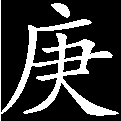
\includegraphics[width=3mm]{../Images/00004}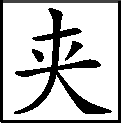
\includegraphics[width=3mm]{../Images/00012}\footnotesize \kaishu 看他刘姥姥笑后复一笑,亦想不到之文也。听宝卿之评,亦千古定论。}惜春道:``都是宝姐姐赞的他越发逞强,这会子拿我也取笑儿。''黛玉忙拉他笑道:``我且问你,还是单画这园子呢,还是连我们众人都画在上头呢?''惜春道:``原说只画这园子的,昨儿老太太又说,单画了园子成个房样子了,叫连人都画上,就像`行乐'似的才好。我又不会这工细楼台,又不会画人物,又不好驳回,正为这个为难呢。''黛玉道:``人物还容易,你草虫上不能。''李纨道:``你又说不通的话了,这个上头那里又用的着草虫?或者翎毛倒要点缀一两样。''黛玉笑道:``别的草虫不画罢了,昨儿`母蝗虫'不画上,岂不缺了典!''众人听了,又都笑起来。黛玉一面笑的两手捧着胸口,一面说道:``你快画罢,我连题跋都有了,起个名字,就叫作《携蝗大嚼图》。''{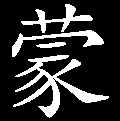
\includegraphics[width=3mm]{../Images/00006}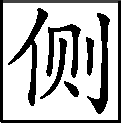
\includegraphics[width=3mm]{../Images/00011}\footnotesize \kaishu 愈出愈奇。}

众人听了,越发哄然大笑,前仰后合。只听``咕咚''一声响,不知什么倒了,急忙看时,原来是湘云伏在椅子背儿上,那椅子原不曾放稳,被他全身伏着背子大笑,他又不提防,两下里错了劲,向东一歪,连人带椅都歪倒了,幸有板壁挡住,不曾落地。众人一见,越发笑个不住。宝玉忙赶上去扶了起来,方渐渐止了笑。宝玉和黛玉使个眼色儿,黛玉会意,{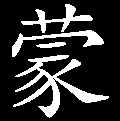
\includegraphics[width=3mm]{../Images/00006}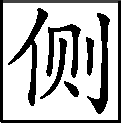
\includegraphics[width=3mm]{../Images/00011}\footnotesize \kaishu 何等妙文心,故意唐突。}便走至里间将镜袱揭起,照了一照,只见两鬓略松了些,忙开了李纨的妆奁,拿出抿子来,对镜抿了两抿,仍旧收拾好了,方出来,指着李纨道:``这是叫你带着我们作针线教道理呢,你反招我们来大顽大笑的。''李纨笑道:``你们听他这刁话。他领着头儿闹,引着人笑了,倒赖我的不是。真真恨的我只保佑明儿你得一个利害婆婆,再得几个千刁万恶的大姑子小姑子,试试你那会子还这么刁不刁了。''{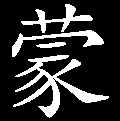
\includegraphics[width=3mm]{../Images/00006}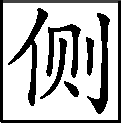
\includegraphics[width=3mm]{../Images/00011}\footnotesize \kaishu 收结转折,处处情趣。}

林黛玉早红了脸,拉着宝钗说:``咱们放他一年的假罢。''宝钗道:``我有一句公道话,你们听听。藕丫头虽会画,不过是几笔写意。如今画这园子,非离了肚子里头有几幅丘壑的才能成画。这园子却是像画儿一般,山石树木,楼阁房屋,远近疏密,也不多,也不少,恰恰的是这样。你就照样儿往纸上一画,是必不能讨好的。这要看纸的地步远近,该多该少,分主分宾,该添的要添,该减的要减,该藏的要藏,该露的要露。这一起了稿子,再端详斟酌,方成一幅图样。第二件,这些楼台房舍,是必要用界划的。一点不留神,栏杆也歪了,柱子也塌了,门窗也倒竖过来,阶矶也离了缝,甚至于桌子挤到墙里去,花盆放在帘子上来,岂不倒成了一张笑`话'儿了。第三,要插人物,也要有疏密,有高低。衣折裙带,手指足步,最是要紧;一笔不细,不是肿了手就是跏了腿,染脸撕发倒是小事。依我看来竟难的很。如今一年的假也太多,一月的假也太少,竟给他半年的假,再派了宝兄弟帮着他。并不是为宝兄弟知道教着他画,那就更误了事;为的是有不知道的,或难安插的,宝兄弟好拿出去问问那会画的相公,就容易了。''

宝玉听了,先喜的说:``这话极是。詹子亮的工细楼台就极好,程日兴的美人是绝技,如今就问他们去。''宝钗道:``我说你是无事忙,说了一声你就问去。等着商议定了再去。如今且拿什么画?''宝玉道:``家里有雪浪纸,又大又托墨。''宝钗冷笑道:``我说你不中用!那雪浪纸写字画写意画儿,或是会山水的画南宗山水,托墨,禁得皴搜。拿了画这个,又不托色,又难滃,画也不好,纸也可惜。我教你一个法子。原先盖这园子,就有一张细致图样,虽是匠人描的,那地步方向是不错的。你和太太要了出来,也比着那纸大小,和凤丫头要一块重绢,叫相公矾了,叫他照着这图样删补着立了稿子,添了人物就是了。就是配这些青绿颜色并泥金泥银,也得他们配去。你们也得另爖上风炉子,预备化胶、出胶、洗笔。还得一张粉油大案,铺上毡子。你们那些碟子也不全,笔也不全,都得从新再置一分儿才好。''惜春道:``我何曾有这些画器?不过随手写字的笔画画罢了。就是颜色,只有赭石、广花、藤黄、胭脂这四样。再有,不过是两支着色笔就完了。''宝钗道:``你不该早说。这些东西我却还有,只是你也用不着,给你也白放着。如今我且替你收着,等你用着这个时候我送你些,也只可留着画扇子,若画这大幅的也就可惜了的。今儿替你开个单子,照着单子和老太太要去。你们也未必知道的全,我说着,宝兄弟写。''

宝玉早已预备下笔砚了,原怕记不清白,要写了记着,听宝钗如此说,喜的提起笔来静听。宝钗说道:``头号排笔四支,二号排笔四支,三号排笔四支,大染四支,中染四支,小染四支,大南蟹爪十支,小蟹爪十支,须眉十支,大着色二十支,小着色二十支,开面十支,柳条二十支,箭头朱四两,南赭四两,石黄四两,石青四两,石绿四两,管黄四两,广花八两,蛤粉四匣,胭脂十片,大赤飞金二百帖,青金二百帖,广匀胶四两,净矾四两。矾绢的胶矾在外,别管他们,你只把绢交出去叫他们矾去。这些颜色,咱们淘澄飞跌着,又顽了,又使了,包你一辈子都够使了。再要顶细绢箩四个,粗绢箩四个,担笔四支,大小乳钵四个,大粗碗二十个,五寸粗碟十个,三寸粗白碟二十个,风炉两个,沙锅大小四个,新磁罐二口,新水桶四只,一尺长白布口袋四条,浮炭二十斤,柳木炭一斤,三屉木箱一个,实地纱一丈,生姜二两,酱半斤。''黛玉忙道:``铁锅一口,锅铲一个。''宝钗道:``这作什么?''黛玉笑道:``你要生姜和酱这些作料,我替你要铁锅来,好炒颜色吃的。''众人都笑起来。宝钗笑道:``你那里知道。那粗色碟子保不住不上火烤,不拿姜汁子和酱预先抹在底子上烤过了,一经了火是要炸的。''众人听说,都道:``原来如此。''

黛玉又看了一回单子,笑着拉探春悄悄的道:``你瞧瞧,画个画儿又要这些水缸箱子来了。想必他糊涂了,把他的嫁妆单子也写上了。''探春``嗳''了一声,笑个不住,说道:``宝姐姐,你还不拧他的嘴?你问问他编排你的话。''宝钗笑道:``不用问,狗嘴里还有象牙不成!''一面说,一面走上来,把黛玉按在炕上,便要拧他的脸。黛玉笑着忙央告:``好姐姐,饶了我罢!颦儿年纪小,只知说,不知道轻重,作姐姐的教导我。姐姐不饶我,还求谁去?''众人不知话内有因,都笑道:``说的好可怜见的,连我们也软了,饶了他罢。''宝钗原是和他顽,忽听他又拉扯前番说他胡看杂书的话,便不好再和他厮闹,放起他来。黛玉笑道:``到底是姐姐,要是我,再不饶人的。''宝钗笑指他道:``怪不得老太太疼你,众人爱你伶俐,今儿我也怪疼你的了。过来,我替你把头发拢一拢。''黛玉果然转过身来,宝钗用手拢上去。宝玉在旁看着,只觉更好,不觉后悔不该令他抿上鬓去,也该留着,此时叫他替他抿去。{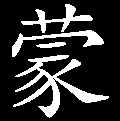
\includegraphics[width=3mm]{../Images/00006}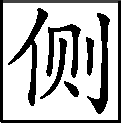
\includegraphics[width=3mm]{../Images/00011}\footnotesize \kaishu 又一点。作者可称无漏子。}正自胡思,只见宝钗说道:``写完了,明儿回老太太去。若家里有的就罢,若没有的,就拿些钱去买了来,我帮着你们配。''宝玉忙收了单子。

大家又说了一回闲话。至晚饭后又往贾母处来请安。贾母原没有大病,不过是劳乏了,兼着了些凉,温存了一日,又吃了一剂药疏散一疏散,至晚也就好了。不知次日又有何话,且听下回分解。

{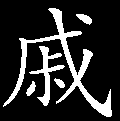
\includegraphics[width=3mm]{../Images/00005} \kaishu 总评:摹写富贵,至于家人女子无不妆点,论诗书,讲画法,皆尽其妙,而其中隐语,惊人教人,不一而足,作者之用心,诚佛菩萨之用心也。读者不可因其浅近而渺忽之。}
